% https://iitdbgroup.github.io/ProvenanceWeek2021/tapp.html

\documentclass[letterpaper,twocolumn,10pt]{article}
\usepackage{usenix-2020-09}

% to be able to draw some self-contained figs
\usepackage{tikz}
\usepackage{amsmath}
\usepackage{tabu}

% inlined bib file
% \usepackage{filecontents}
% 
% %-------------------------------------------------------------------------------
% \begin{filecontents}{\jobname.bib}
% %-------------------------------------------------------------------------------
% %
% %
% %
% \end{filecontents}

%-------------------------------------------------------------------------------
\begin{document}
%-------------------------------------------------------------------------------

% don't want date printed
\date{}

% make title bold and 14 pt font (Latex default is non-bold, 16 pt)
\title{\Large \bf A multi-system provenance architecture based on PROV-DM for Explainable AI: Application Track}

% for single author (just remove % characters)
\author{
{\rm Nicholas J. Car}\\
SURROUND Pty Ltd \&\\
Australian National University\\
\href{mailto:nicholas.car@surroundaustralia.com}{nicholas.car@surroundaustralia.com} 
\and
{\rm Robert A. Atkinson}\\
SURROUND Pty Ltd \&\\
Open Geospatial Consortium\\
\href{mailto:rob.atkinson@surroundaustralia.com}{rob.atkinson@surroundaustralia.com} 
} % end author

\maketitle

%-------------------------------------------------------------------------------
\begin{abstract}
%-------------------------------------------------------------------------------
% CFP: https://iitdbgroup.github.io/ProvenanceWeek2021/cfp.html
% Applications Track: need not to focus on novelty but should instead focus on innovative use of provenance and/or deployment of provenance-based solutions and/or open-source software. We invite authors to share insights, experience, and lessons learned when deploying provenance systems. We also encourage submissions describing datasets or tools that could benefit the community.

% Structure: insights, experience, and lessons learned when deploying provenance systems
SURROUND Australia Pty Ltd is a small technology company focused on explainable 
AI and knowledge management products. At the core of our company operations is 
standardised provenance tracking using the PROV Data Model (PROV-DM). Using standardised 
provenance throughout our company lets us both assure customers that any results 
we produce for them are explainable, regardless of the specific systems we employ, 
and also allows us to supply provenance tooling to clients that will work well 
with other logging or provenance systems.

We generate PROV-DM-based provenance in all our important business workflows by 
using either our in-house \textit{ProvWF} tool or workflows within our 
proprietary \textit{SURROUND Ontology Platform} tool. We implement PROV-DM within our 
Knowledge Graph (KG) data products, which are a major part of our business, through the 
\textit{SURROUND Ontology Platform} also and we ''hand off'' provenance tracking 
of some objects to the Git version control system. Our various workflows' and KGs' provenance
information is used together to provide explainable AI results.
\end{abstract}


%-------------------------------------------------------------------------------
\section{Introduction}
%-------------------------------------------------------------------------------
SURROUND Australia Pty Ltd (``SURROUND'') is a small technology company founded 6 years ago. While
aiming to supply mainstream AI and knowledge management products to government and private
sector markets, SURROUND attempts to distinguish itself from competitors through sophisticated use
of Semantic Web data due to the belief that such data is the form that best preserves meaning 
over time and system \& organisational change. Specific value propositions for SURROUND's customers, 
based on Semantic Web data use, are:

\begin{itemize}
  \item the expressive power of RDF Schema and OWL2~\cite{dan_brickley_rdf_2014,w3c_owl_working_group_owl_2012} for complex data modelling
  \item the ability to reuse many existing, sophisticated, publishd ontologies directly
  \item the extensibility of RDF graph-based data structures
  \item the systems-independence of Semantic Web data formats
  \item the ability to use a Semantic Web layer to act as a bridge between internal, siloed applications
  \item the ability to share data across organisational boundaries with no inter-organisational special data contracts (due to semantic modelling of all data elements)
  \item the data validation power of modern constraints languages such as SHACL~\cite{knublauch_shapes_2017}
  \item the advanced reasoning capabilities of OWL \& SHACL
\end{itemize}

Emergent from some of these points is SURROUND's ability to provide comensurate provenance information 
across all our different systems due to them all implementing the PROV Data Model (PROV-DM)~\cite{moreau_prov-dm_2013}
in its ontology form, PROV-O~\cite{lebo_prov-o:_2013}, and our ability to produce PROV-O data, to share 
it between applications, to store it and present it.

In this paper we make no new research claim - this is an \textit{Applications Track} paper - but we do aim 
to show ``innovative use of provenance'' and ``the deployment of provenance-based solutions'' that indicate
a certain maturity of approach to the use of provenance for operational tasks. We expect this will be of 
interests to our industry peers and to academics wishing to know where industry implementers are up to
in order to consider next research steps.

We will overview our specific company-wide provenance systems, discuss two projects that use them, indicate 
why we've chosen certain PROV-related implementations over others and where we think some of the provenance
standards need enhancement for our purposes.


%-------------------------------------------------------------------------------
\section{Simple enough theory, complex practice}
%-------------------------------------------------------------------------------
Extraction of useful information present within heterogeneous or large-scale data contexts may be performed in several 
ways. If some of the data has some known structure then queries can be used to select relevant subsets. The trivial form 
of this is searching against text content, with various degrees of sophistication. These may involve statistical 
techniques to identify patterns in the data. SURROUND uses Machine Learning (ML) approaches to train systems to correlate or 
discover information based on various patterns. We also use Semantic or Knowledge Graph-based contextual information to 
assist such processes to improve performance. Conversely, we also use ML approaches to infer structure. Some of our projects
include Human-in-the-loop (HITL) activities too, to refine, record and improve training of systems. Performing these tasks 
requires us to implement complex, hybrid systems that use reasoning and ML to create ways to to organise and retrieve 
information from complex projects, two of which are summarised in the next sections.  

The role of provenance for us within these systems is twofold: firstly so that we can provide our customers certainty of project 
outputs, and scondly so that we can track our systems performance so we can improve our offerigs over time. The challenge 
is that many, very different, types of systems interact, and so to provide end-to-end provenance for customers and ourselves
that is usable, we have to pay close attention to the provenance models use across all of them and their technical integration.

From the theoretical perspective, this is simple and facilitated by PROV-DM acting as canonical model for provenance which SURROUND
applies ``everywhere'' (as far as we practically can). The practical challenges are still significant though and can be 
characterised as being of two main types:

\begin{enumerate}
  \item \textbf{Shared entity identification} - making sure different systems can use the same identifiers for entities as they pass between systems
  \item \textbf{Granularity} - having useful levels of detail about pieces of knowledge whilst retaining ability to have overviews from the process level and support large scale batch processing
\end{enumerate}

Shared entity identification is well handled using the RDF meta model, which uses unique URIs for things (entities and others) and 
the Open World Assumption, as multiple systems can represente knowledge in RDF data structures and then join knowledge by referencing 
shared URIs. SURROUND not only communicates our provenance infromation in RDF but, for most projects, our primary data also. Since 
our primary data, perhaps electronic records described using RDF metadata, and our provenance information describing that data's 
generation are both represented in RDF, we can identify entities across both information holdings too, not just across sytems within 
each holding.

Architecturally, our primary project data an our provenance can be integrated across multiple subsystems if:

\begin{enumerate}
  \item Object identity is established as part of KG management and accessed via APIs from this shared body of knowledge when required
  \item Object identity is managed within the KG whenever ``human in the loop'' interactions are required
  \item Processing subsystems preserve and report canonical object identities
  \item Coherent sets of objects may be managed in specialised persistence systems, as long as the description of data set itself and access mechanisms are part of the knowledge graph (data set granularity)
  \item All processing reports provenance along with outputs using a canonical model
  \item Processing elements are identified in the knowledge graph in a coherent way
\end{enumerate}

Figure~\ref{fig:sankey} shows the user interface of the \textit{SURROUND Ontology Platform} (SOP) displaying provenance information within 
a sankey diagram. The provenance information was generated according to PROV-DM/PROV-O by SURROUND's processing workflow tool \textit{ProvWF} 
which, in the displayed instance, performed Named Entity Recognition against electronic records using cloud-hosted scalable services and some 
of SURROUND's Knowledge Graph products for entity matching. In addition to displaying the provenance information in particular ways, SOP also 
managed is in bundles as \textit{Managed Graphs} whihc, from SOP's point of view are yet another semantic asset for which provenance (and 
ownershi, access etc.) is automatically stored.

%-------------------------------------------------------------------------------
\begin{figure*}
  \begin{center}
    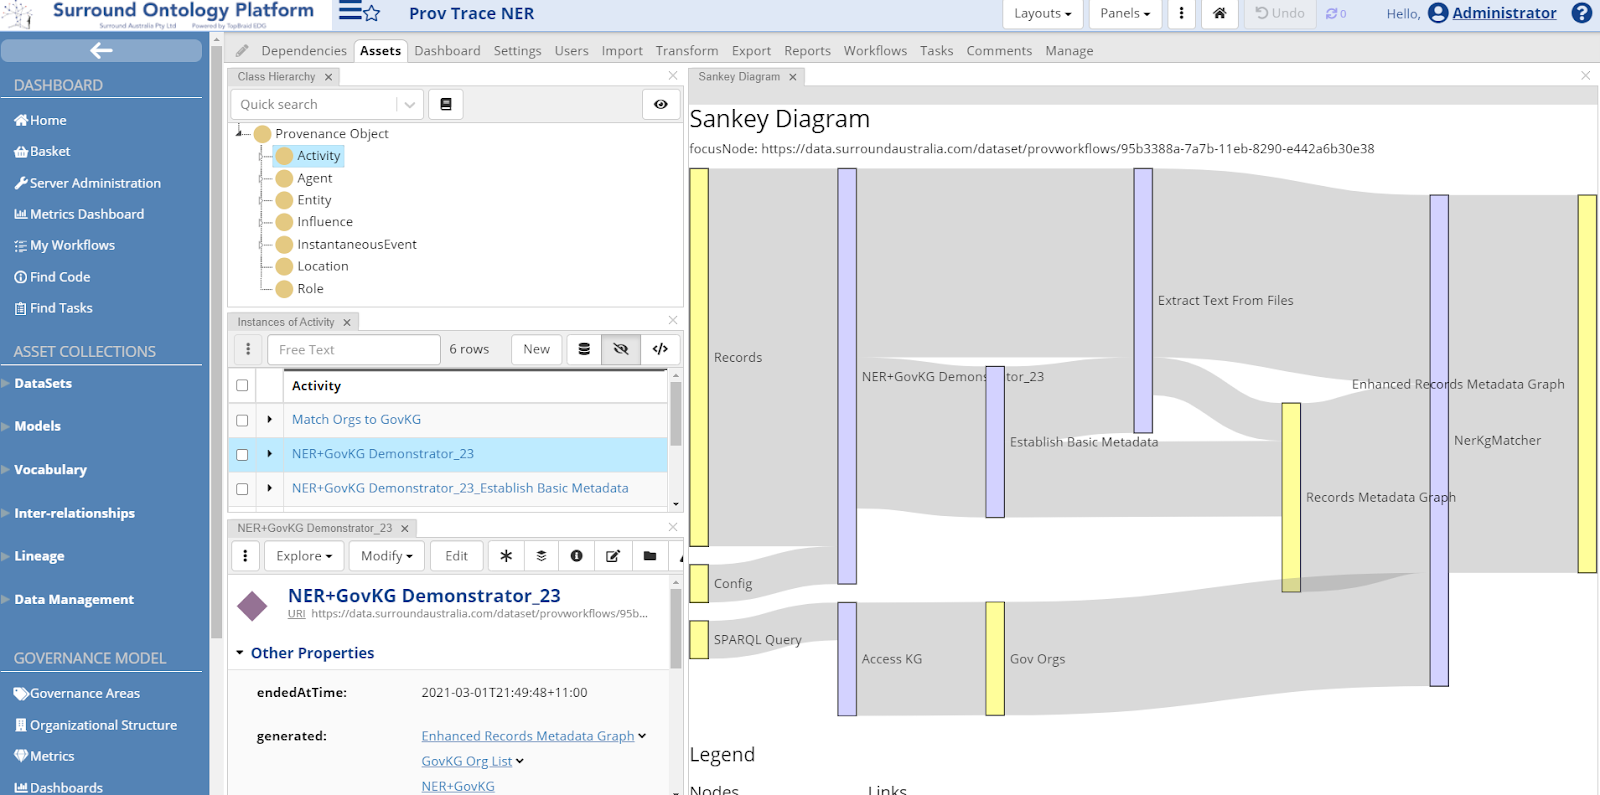
\includegraphics[width=\textwidth]{images/sankey.png}
  \end{center}
  \caption{\label{fig:sankey} An example of a provenance trace from a processing workflow that uses elements of a knowledge graph, performs processing in cloud-hosted scalable services, generates augmented views of an input stream (performing Named Entity Recognition on a document set and annotating with elements from the knowledge graph), persists the results in the knowledge graph and integrates the provenance trace with the provenance trace generated by knowledge graph management.}
  \end{figure*}
%-------------------------------------------------------------------------------

The provenance granularity issue identified above can be summarised by examining a range of different types of processing that may typically 
occur in a heterogeneous system, perhaps one performing ML to augment a knowledge base. Table X

\begin{table*}[t]
  \centering
  \begin{tabular}{|p{5cm}|p{5cm}|p{5cm}|}
    \hline
    \textbf{Function} & \textbf{Examples} & \textbf{Granularity}\\
    \hline
    Human-in-the-loop & Establishment of definitions, Registration of individual entities, Annotation, Classification for training & Statement, Reified statements\\ 
    \hline
    Database management, Data transformation & Making a set of data instances available to a knowledge base in a useful form & Data set (table, spreadsheet, graph etc)\\ 
    \hline
    Query & Extraction of data subsets & Data set, Result set\\
    Governance & & Data set\\
    \hline
    Bulk document processing & Indexing, classification, clustering & Container (directory, database, storage bucket etc)\\
    \hline
    Document analysis & Making information elements in a document available to finer grained processes & Document, derived data set\\
    \hline
    Knowledge Graph Management & Establishment of a known state of complex, modular knowledge graphs, Capture of provenance, Support for automated updates & Graph (Data set)\\
    \hline
  \end{tabular}
  \caption{Blabla}
  \label{tab:1}
\end{table*}



%-------------------------------------------------------------------------------
\section{Company-wide provenance architecture}
%-------------------------------------------------------------------------------
SURROUND has a company-wide policy on provenance which is simple that \textit{all} project data processing 
and system operations for clients - work on demand or services supplied - must be recorded in 
PROV-O-compliant forms, with the exception of code and data stored in version control systems which, in all 
instances so far, are implemented in Git\footnote{Git is a free and open source distributed version control 
system, see \url{https://git-scm.com/}}. So far, this policy has been implemented for all our main projects' 
systems and processes, but not for minor projects, some legacy systems or administrative support functions.

Figure~\ref{fig:overview} links types of IT project assets we work with for clients to the tools we implement
to record PROV-O-compliant provenance. 

%-------------------------------------------------------------------------------
\begin{figure*}
  \begin{center}
    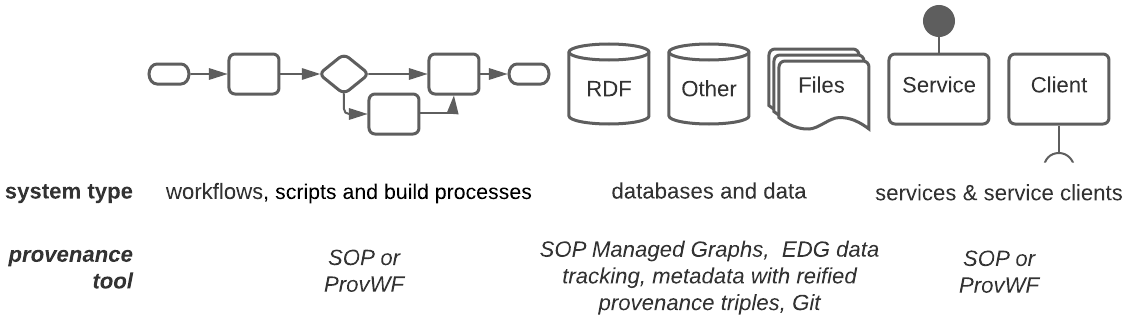
\includegraphics[width=\textwidth]{images/overview.png}
  \end{center}
  \caption{\label{fig:overview} SURROUND's provenance tools linked to system type}
  \end{figure*}
%-------------------------------------------------------------------------------

Our major provenance tools, as named in Figure~\ref{fig:overview}, and the actions they perform are:

\begin{itemize}
  \item \textbf{SURROUND Ontology Platform} (SOP)\footnote{\url{https://surroundaustralia.com/sop}}
  \begin{itemize}
    \item an enterprise data management system based on sematic data that is based on Top Quadrant's \textit{EDG}\footnote{\url{https://www.topquadrant.com/products/topbraid-enterprise-data-governance/}}
    \item SOP extends EDG adding the ability to manage various types of semantic assets and collections of them
    \item SOP records PROV-DM provenance for all semantic asset actions
  \end{itemize}
  \item \textbf{ProvWorkflow} (ProvWF)\footnote{\url{https://surroundaustralia.com/provwf}}
  \begin{itemize}
    \item a Python framework and library for the creation of workflows
    \item records PROV-DM provenance for all actions performed by the workflow and all data consumed or produced
    \item supported by SURROUND's \textit{Block Library}
  \end{itemize}
  \item \textbf{Block Library}
  \begin{itemize}
    \item SURROUND's catalogue of ProvWF \textit{Blocks} which are PROV-DM \texttt{Activity} class objects
    \item the library stores many reusable functions within \textit{Blocks}, such as Knowledge Graph API requests, NLP text processing etc.
  \end{itemize}
  \item \textbf{Git}
  \begin{itemize}
    \item we use Git to track the versions of many assets - code, data etc. - in both public and private repositories
    \item although we know of Git-to-PROV mapping tools, e.g. Git2PROV~\cite{tom_de_nies_git2prov_nodate}, we have not yet found it necissary to materialise such mappings but instead record identifiers for versions of PROV-DM \texttt{Entities} using Git and refer to them in PROV-O data
  \end{itemize}\item 
\end{itemize}

In addition to these provenance-specific tools, we implement provenance tracking with general-purpose tools too, such as:

\begin{itemize}
  \item \textbf{RDFlib} (SOP)\footnote{\url{https://github.com/RDFLib/rdflib}}
  \begin{itemize}
    \item a general-purpose RDF manipulation library, written in Python
    \item many of our data objects are RDF graphs
    \item used to create reified provenance for RDF statements     
  \end{itemize}
\end{itemize}  

We ensure provenance information generated by one of our tool is usable in another, for example, \textit{ProfWF}'s outputs
can, and often are, stored in \textit{SOP} which is then able to visualise that provenance either in isolation order
by joining it to other provenance information, perhaps captured by \textit{SOP} itself.


%-------------------------------------------------------------------------------
\begin{figure*}
  \begin{center}
    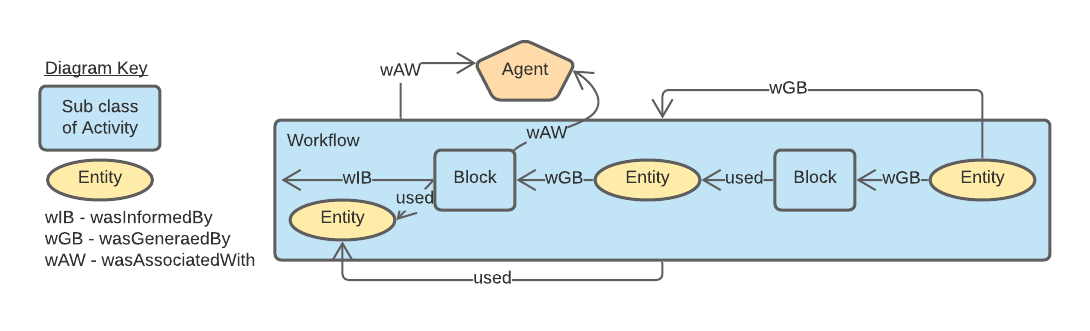
\includegraphics[width=\textwidth]{images/provwf.png}
  \end{center}
  \caption{\label{fig:provwf} An example of the main PROV-O elements generated by \textit{ProvWF}. Note that the tooling automatically captures identifiers for the versions of software used for any particular workflow implementatation}
  \end{figure*}
%-------------------------------------------------------------------------------

%-------------------------------------------------------------------------------
\begin{figure*}
  \begin{center}
    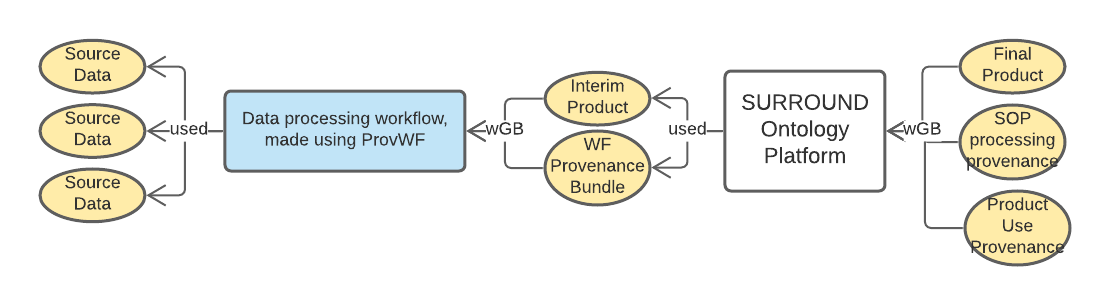
\includegraphics[width=\textwidth]{images/provwf-to-sop.png}
  \end{center}
  \caption{\label{fig:provwf-to-sop} \textit{ProvWF} is often used to generate RDF data - here the ``Interim Product'' - which can be supplied to \textit{SOP} with an acompanying provenance \texttt{Bundle}. \textit{SOP}, in turn, generates both \texttt{Bundles} of provenance for any actions on data it performs and also recurds usage provenance for products}
  \end{figure*}
%-------------------------------------------------------------------------------

%-------------------------------------------------------------------------------
\begin{figure*}
  \begin{center}
    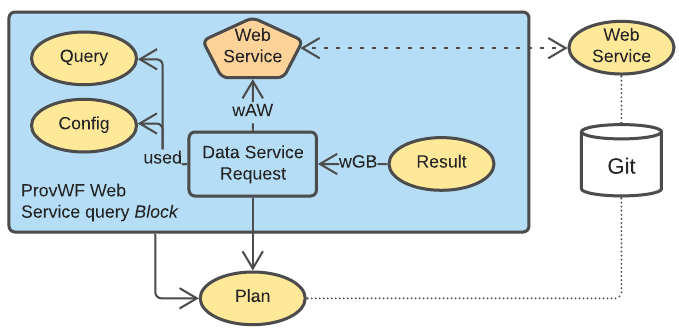
\includegraphics[width=\textwidth]{images/data-service.png}
  \end{center}
  \caption{\label{fig:data-service} SURROUND's provenance tools linked to system type}
  \end{figure*}
%-------------------------------------------------------------------------------

%-------------------------------------------------------------------------------
\begin{figure*}
  \begin{center}
    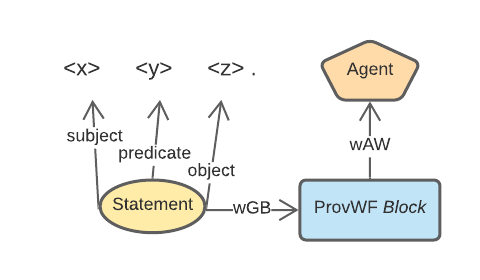
\includegraphics[width=\textwidth]{images/reified-graph-data.png}
  \end{center}
  \caption{\label{fig:reified-graph-data} SURROUND's provenance tools linked to system type}
  \end{figure*}
%-------------------------------------------------------------------------------



%-------------------------------------------------------------------------------
\section*{Availability}
%-------------------------------------------------------------------------------

USENIX program committees give extra points to submissions that are
backed by artifacts that are publicly available. If you made your code
or data available, it's worth mentioning this fact in a dedicated
section.

%-------------------------------------------------------------------------------
\bibliographystyle{plain}
% \bibliography{\jobname}
\bibliography{TaPP21}

%%%%%%%%%%%%%%%%%%%%%%%%%%%%%%%%%%%%%%%%%%%%%%%%%%%%%%%%%%%%%%%%%%%%%%%%%%%%%%%%
\end{document}
%%%%%%%%%%%%%%%%%%%%%%%%%%%%%%%%%%%%%%%%%%%%%%%%%%%%%%%%%%%%%%%%%%%%%%%%%%%%%%%%

%%  LocalWords:  endnotes includegraphics fread ptr nobj noindent
%%  LocalWords:  pdflatex acks
